\documentclass[11pt]{article}

\usepackage{graphicx}

\oddsidemargin=.25in
\evensidemargin=.25in
\textwidth=6in
\topmargin=0in

\parindent=0in

\begin{document}

\centerline {\Large \bf Kobby Editor: Collaborative Editing Instructions}
\centerline {Written by Gregory Haynes}

\paragraph{}The central feature of Kobby is the ability to host and join collaboratively edited documents.  Collaborative editing allows multiple people to work on the same document simultaneously, similar to how several people could write on a large sheet of paper simultaneously.

\begin{figure}[tbh]
\begin{center}
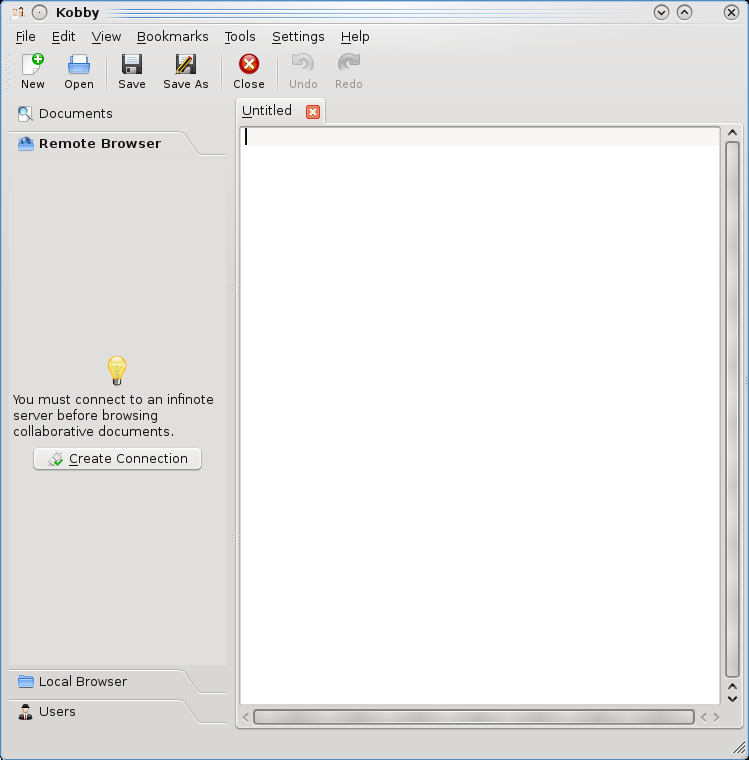
\includegraphics[width=.7\textwidth]{kobbymain.png}
\end{center}
\caption{Kobby Editor Main Window}
\end{figure}

\paragraph{}Collaborative editing in Kobby is done by having each document ``hosted'' on one persons computer, while all the other users connect to that computer and edit the same document.  Thinking in terms of the drawing on paper example, in order for everyone to draw on the same paper everyone must agree on which sheet of paper will be used.  Once a document has been created on the host computer, users can then join the document to begin editing.  This instruction will walk through the process of creating a document on a host computer, and then joining that document to begin collaborative editing.

\paragraph{Before you begin} Before using these instructions, you must have a recent version of Kobby installed on your computer.  If you do not know how to install Kobby, instructions for doing this can be found on the Kobby website at http://greghaynes.github.com/kobby.

\paragraph{Starting the server} In order to collaboratively edit documents, you must have a document host you can connect to.  Think of this host as the person who is physically holding all the documents.  Users who connect to this host can be thought of as other people asking the holder to work on his/her documents.  If you do not already have a host to connect to, you can start a server and act as a host yourself.

\begin{figure}[tbh]
\begin{center}
 \includegraphics[width=.85\textwidth]{infinotedterm.png}
\end{center}
\caption{Starting the collaborative document server}
\end{figure}

{\bf Start the Collaborative Document Server/Host:}\\
\begin{enumerate}
 \item Open a terminal on your computer.
 \begin{itemize}
  \item If you do not know how to open a terminal, consult your computer's software manual.
 \end{itemize}
 \item Enter the following command into your terminal and execute it (usually done by pressing [Enter] or [Return]).  An example of this can be seen in figure 2.
 \begin{quote}
  infinoted-0.3 --security-policy=no-tls
 \end{quote}
 \item Your server should now be running.  Now you can move on to Connecting to a Server.
\end{enumerate}

\paragraph{Connecting to a server} Once you know what host to connect to (localhost if you are running your own server as in the above instructions), you can start the collaborative editing process by connecting to the host. \\

\begin{figure}[tbh]
\begin{center}
 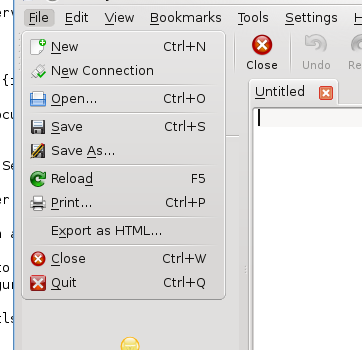
\includegraphics[width=.4\textwidth]{kobbyfilemenu.png}
\end{center}
\caption{Kobby's File Menu}
\end{figure}

\begin{figure}[tbh]
\begin{center}
 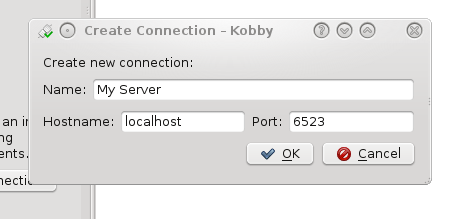
\includegraphics[width=.6\textwidth]{kobbyconnection.png}
\end{center}
\caption{Create Connection Dialog}
\end{figure}

{\bf Connecting to a collaborative server:}\\
\begin{enumerate}
 \item From the ``File'' menu select ``New Connection'', just as shown in figure 3.
 \begin{itemize}
  \item Once you select the ``New Connection'' item, a ``Create Connection'' dialog should appear, as shown in figure 4.
 \end{itemize}
 \item Enter a name of your choice for the connection in the text box labeled Name, and the hostname of the server you are connecting to.  If you are running your own server (as in the ``Starting the Server'' instructions, your hostname is localhost).  This is shown in figure 4.
 \item Once you have entered this information, click connect.
 \item After you have clicked connect, the ``Remote Browser'' box on the left side of the Main Window should show your new connection, as shown in figure 5.
\begin{figure}[tbh]
\begin{center}
 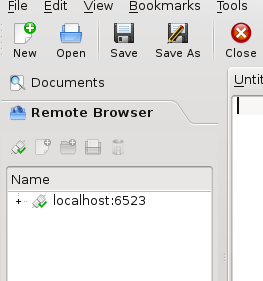
\includegraphics[width=.4\textwidth]{kobbylocalhostconnection.png}
\end{center}
\caption{Connected to the server}
\end{figure}
 \item Select the `+' symbol to the left of the newly created connection.  This plus symbol is how you will browse the folders on the server.
 \item Select the line under the new connection with a folder icon and a '/'.
 \item Now select the Document icon that has a plus sign in the top right corner.  It is located on the toolbar above the newly created connection.  This is how you can create new documents on the server.
 \item Once you click this icon, a dialog should appear to enter the new documents name.  Chose a name for this document, like ``Test'' and click ``Ok''.
 \item This new document should now appear in the left ``Remote Browser'' section, under the already selected ``/'' folder.  Double click on this document to begin editing it.
\end{enumerate}

You should now be able to edit the document just like in any other text editor.  Other users should also be able to join the document just as you have and watch everything being typed into the other users' editors.

\end{document}
